\documentclass[12pt,a4paper]{article}
\usepackage{styles}

\lstset{style=sharpc, tabsize=1}

\renewcommand{\sectionbreak}{\clearpage}

\author{Alexander van Schie \& Oli Dias}
\title{Gruppenarbeit 1 - Cloud Fundamentals beim Provider}
\begin{document}
\maketitle
\newpage
\tableofcontents
\newpage
\section{Hands-On: Hello (Cloud) World}
Dieses Kapitel befasst sich mit der ersten Erfahrung mit dem gewählten Cloud Provider: Openshift Online. 

Die Wahl ist nach einer kurzen Recherche auf Openshift gefallen, weil die ausgedachten Kriterien (Verknüpfung mit GitHub Repository, Push auf Repo führt zu Redeploy und .NET Core und Java Spring Kompatibiltät) mit dem ersten Eindruck effizient vollbracht werden können. 
%TODO Einleitung schreiben mit erklärung wieso, Start Stopp Möglichkeiten, Logfilesls, Vorteil/Nachteil ggü Google App Engine
\subsection{Installationsanleitung}
Das Ziel ist es, eine ASP.NET-Core Hello-World Applikation mittels Openshift Online zu builden und deployen. Am Schluss dieser Installationsanleitung sollte dies möglich sein.


Für das Deplyoment dieser Applikation auf der Openshift Online Plattform müssen grob folgende Schritte durchgeführt werden:
\begin{itemize}
	\item Account und Projekt auf der Plattform erstellen
	\item GitHub Repository der ASP.NET-Core Applikation mit Openshift Projekt verbinden
	\item Applikation auf Openshift builden
	\item Applikation auf Openshift deployen
\end{itemize}
\subsubsection{Openshift Account erstellen}
Zuerst muss ein Account auf  \url{https://manage.openshift.com/signin} erstellt werden. Danach kann zwischen den in Abbildung \ref{fig:openshift-plan} vorgeschlagenen Plänen ausgewählt werden. Wir benutzen den Openshift Online Pro Plan (30-day trial).
\begin{figure}[h]
	\centering
	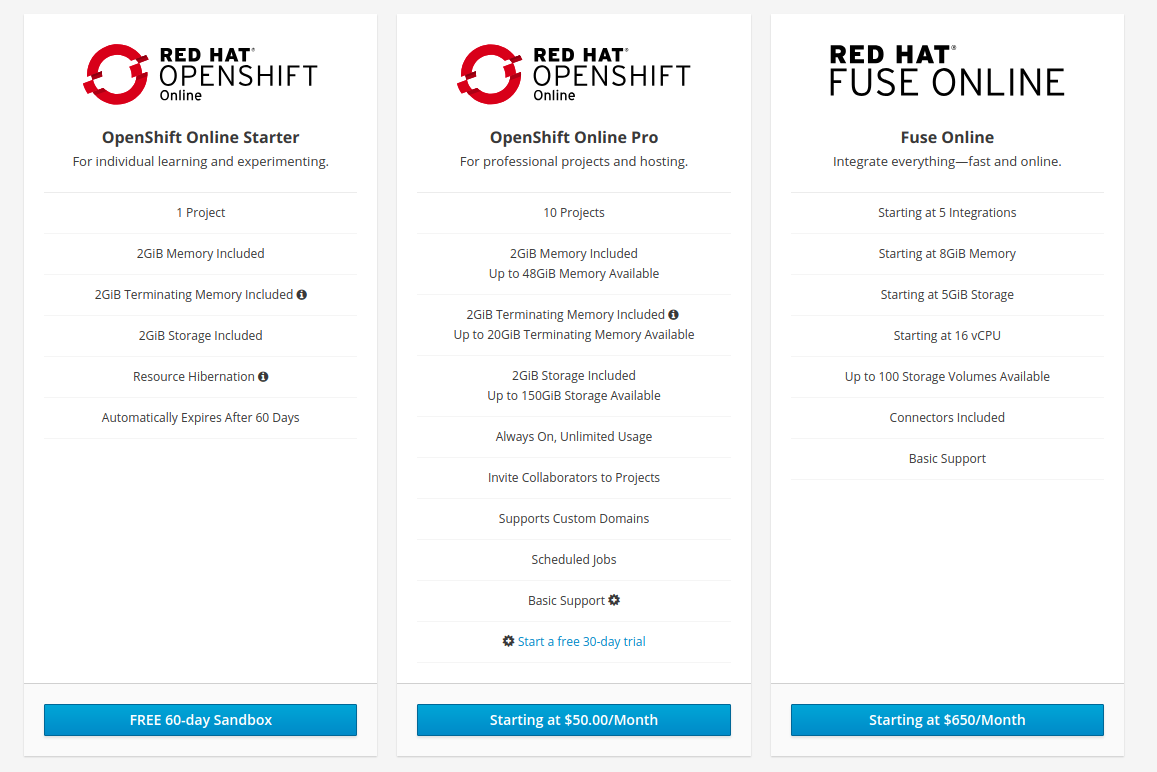
\includegraphics[width=0.7\linewidth]{img/openshift-plan}
	\caption{Gewählter Plan Openshift}
	\label{fig:openshift-plan}
\end{figure}

Dass der Account verifiziert werden kann, muss eine Telefonnummer hinterlegt werden, auf welche darauffolgend einen Bestätigungscode zugeschickt wird. 

Wurde diese eingegeben und verifiziert, erscheint eine Übersicht über das bestellte Produkt wie in Abbildung \ref{fig:os-overview} angezeigt. Daraufhin kann die Subscription bestätigt werden.

\begin{figure}
	\centering
	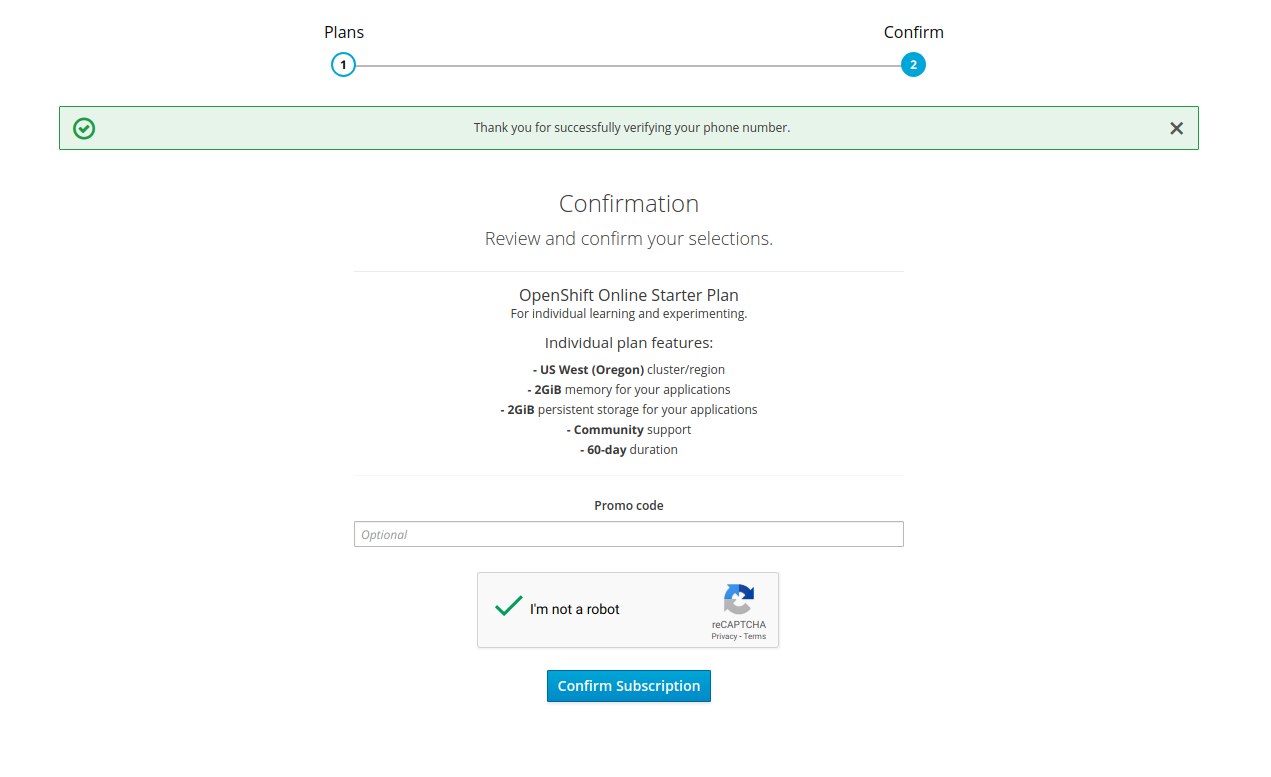
\includegraphics[width=0.9\linewidth]{img/os-overview}
	\caption{Übersicht des abgeschlossenen Plans}
	\label{fig:os-overview}
\end{figure}
Kurz nach dem Bestätigen sollte ein Bestätigungsmail eintreffen. Darauffolgend kann bereits die Web Console geöffnet werden. Es wird ein Katalog mit allen Produkten von Openshift Online dargestellt (Abbildung \ref{fig:os-overview-catalog}).

\begin{figure}[h]
	\centering
	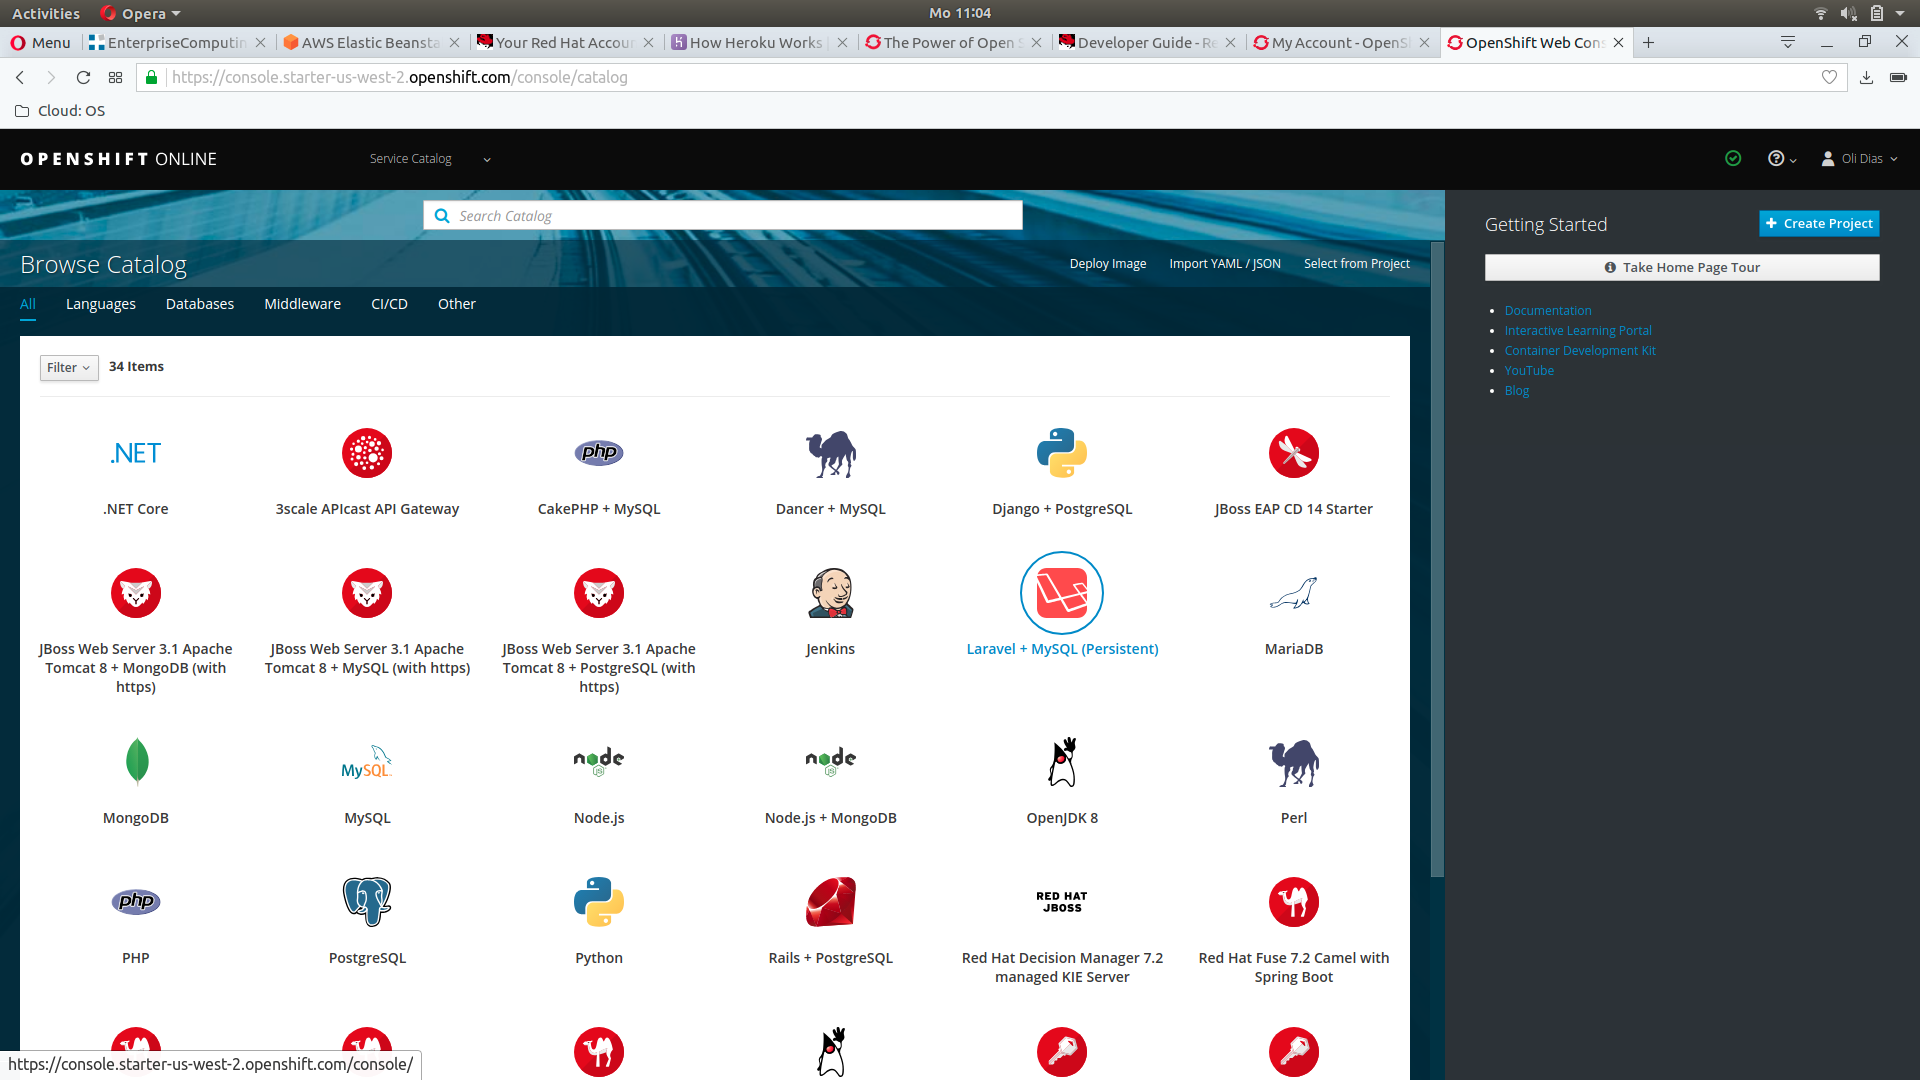
\includegraphics[width=0.7\linewidth]{img/os-overview-catalog}
	\caption{Katalog von Openshift}
	\label{fig:os-overview-catalog}
\end{figure}
Das Erstellen des Openshift Accounts ist somit abgeschlossen und die Platt\-form ist für das Builden und Deployen von Applikationen bereit. 


\subsubsection{Build und Deployment der Applikation mit dem Web-UI}\label{sec:net-webui}
In der Web-Console können wir nun auf .NET Core Projekt klicken. Daraufhin erscheint ein Wizard, dem wir Schritt für Schritt folgen können. Falls das GitHub-Repository schon während dem Wizard hinzugefügt werden soll, muss es bereits existieren und sichtbar sein. 

Entsprechende Felder müssen gemäss Abbildung \ref{fig:os-new-config} ausgefüllt sein. Vorsicht ist bei der .NET Version geboten; wir verwenden die Version 2.2 von .NET Core. 
\begin{figure}[h]
	\centering
	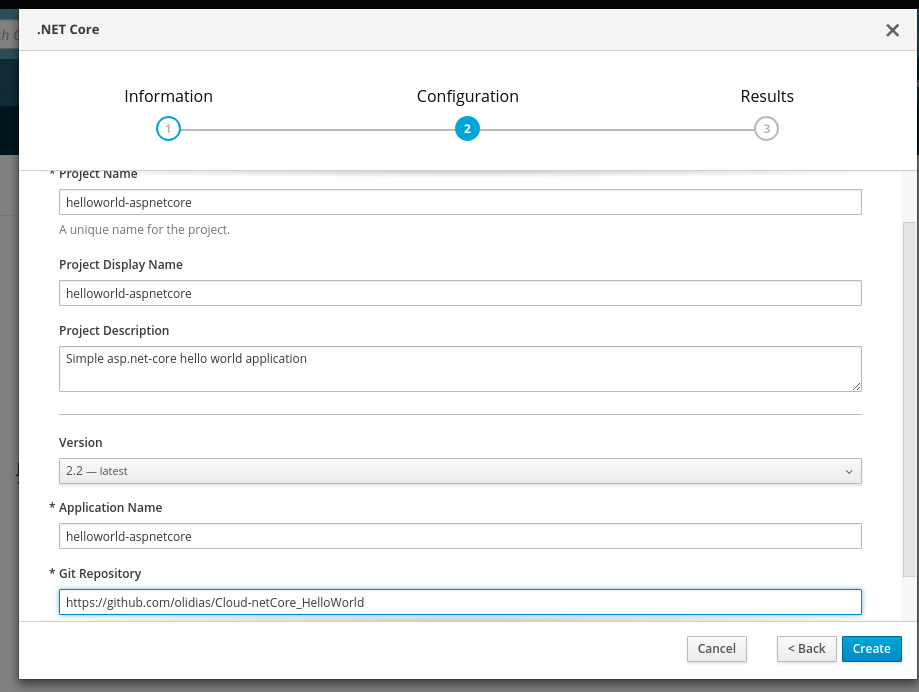
\includegraphics[width=0.7\linewidth]{img/os-new-config}
	\caption{Konfiguration des neuen Projektes}
	\label{fig:os-new-config}
\end{figure}

Sobald das Projekt in Openshift erstellt wurde, startet der Build. 
\begin{figure}[h]
	\centering
	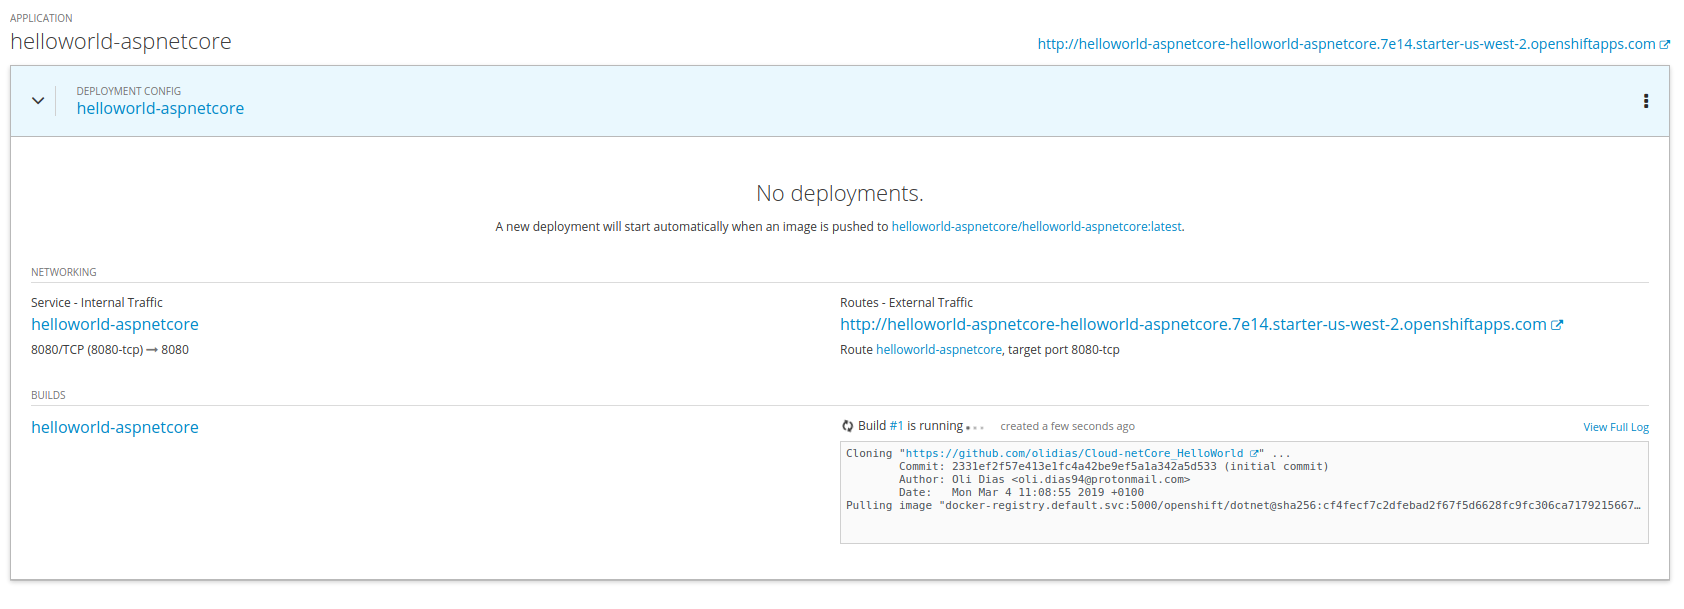
\includegraphics[width=0.7\linewidth]{img/os-building}
	\caption{Builden der .NET Core Applikation}
	\label{fig:os-building}
\end{figure}
Womöglich schlägt der Build aufgrund fehlender \texttt{.s2i}-Konfiguration (Source-2-Image) fehl. Um diesen Fehler zu beheben, muss Openshift gesagt werden, wo das Startup-Projekt liegt. Dazu muss ein Ordner und File mit dem Namen \texttt{.s2i/environment} erstellt werden. Dieses beinhaltet folgendes:
\begin{lstlisting}[breaklines=true]
DOTNET_STARTUP_PROJECT=HelloWorld-netcore/HelloWorld-netcore.csproj
\end{lstlisting}
Wichtig ist weiter zu beachten, dass die .NET Version mit derjenigen von Openshift kompatibel ist.

War der Build erfolgreich, muss noch das Deployment konfiguriert werden. Dazu kommt ein weiteres File mit dem Namen \texttt{run} ins \texttt{.s2i} Verzeichnis. Darin muss die Applikation noch gestartet werden. Dies funktioniert so:
\begin{lstlisting}
exec dotnet run
\end{lstlisting}
Ist auch dieser Schritt vollbracht und der Build erfolgreich, kann im Control Panel des Projektes zu Deployments $\rightarrow$ Routes navigiert werden. Dort erscheint eine Tabelle, wo der Hostname bereits angegeben ist und womit nun die ASP.NET-Core Applikation vom Internet her erreichbar ist.



\subsubsection{Installation der Openshift CLI}
Neben dem Web-UI besteht ähnlich wie mit GAE die Möglichkeit, ein Konsolentool für das Konfigurieren der Cloud Projekte zu verwenden. Die Installation des Tools stellte auf Ubuntu 18.04 LTS ein Problem dar, wie im Folgenden beschrieben wird. 

Beim Ausführen der Konsolenapplikation \texttt{oc}, auf die in der Doku \footnote{\url{https://docs.openshift.com/online/getting_started/basic_walkthrough.html}} verwiesen wird, kam der Fehler in Abbildung \ref{fig:oc-error} auf.

\begin{figure}[h]
	\centering
	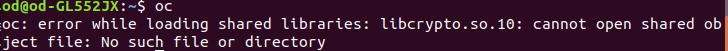
\includegraphics[width=1\linewidth]{img/oc-error}
	\caption{Fehler beim Ausführen des OC}
	\label{fig:oc-error}
\end{figure}

Gemäss einem Issue auf GitHub\footnote{\url{https://github.com/openshift/origin/issues/21061}} handelt es sich um einen fehlerhaften Symlink, der in dieser spezifischen Version enthalten war. Es wird des Weiteren auf eine aktueller Version verwiesen, mit welcher das Problem nicht mehr existiert. Openshift garantiert nur für RHEL\footnote{Red Hat Enterprise Linux} Support, weshalb auf anderen Linux Distributionen oder Betriebssystemen mit solchen Fehlern gerechnet werden muss.


\subsubsection{Build und Deployment der Applikation mit dem CLI}

Nachdem die Installation des CLI vollbracht ist, können die gleichen Befehle des Web-UIs in der Konsole ausgeführt werden. 
\begin{description}
	\item[Erstellen eines Projektes] \hfill\\
	\texttt{oc new-project helloWorld --display-name='ASP.NET Core Hello World'}
	\item[]
\end{description}
\section{Analyse: OSSM-Definition}

Damit sich jemand als Cloud Computing Provider ausgeben kann, sollten folgende Chrakteristiken erfüllt sein:

\begin{itemize}
	\item On-demand
	\item Self-service
	\item Scalable
	\item Measurable
\end{itemize}

In den folgenden Kapiteln erläutern wir, wie Openshift diese umsetzt.

\subsection{On-demand \& Self-service}

Auf der Startseite findet man eine Katalog aller möglichen Projekttypen. Nach einem Klick auf den gewünschten Projekttyp erscheint ein Dialog, in welchem die spezifische Konfiguration vorgenommen werden kann. Gleichzeitig wird geprüft, ob die definierte Konfiguration plausibel ist. Ist dies der Fall, kann das Projekt erstellt werden.
Nach wenigen Sekunden ist das Projekt unter der Rubrik "My Projects" ersichtlich.

\begin{figure}[h]
	\centering
	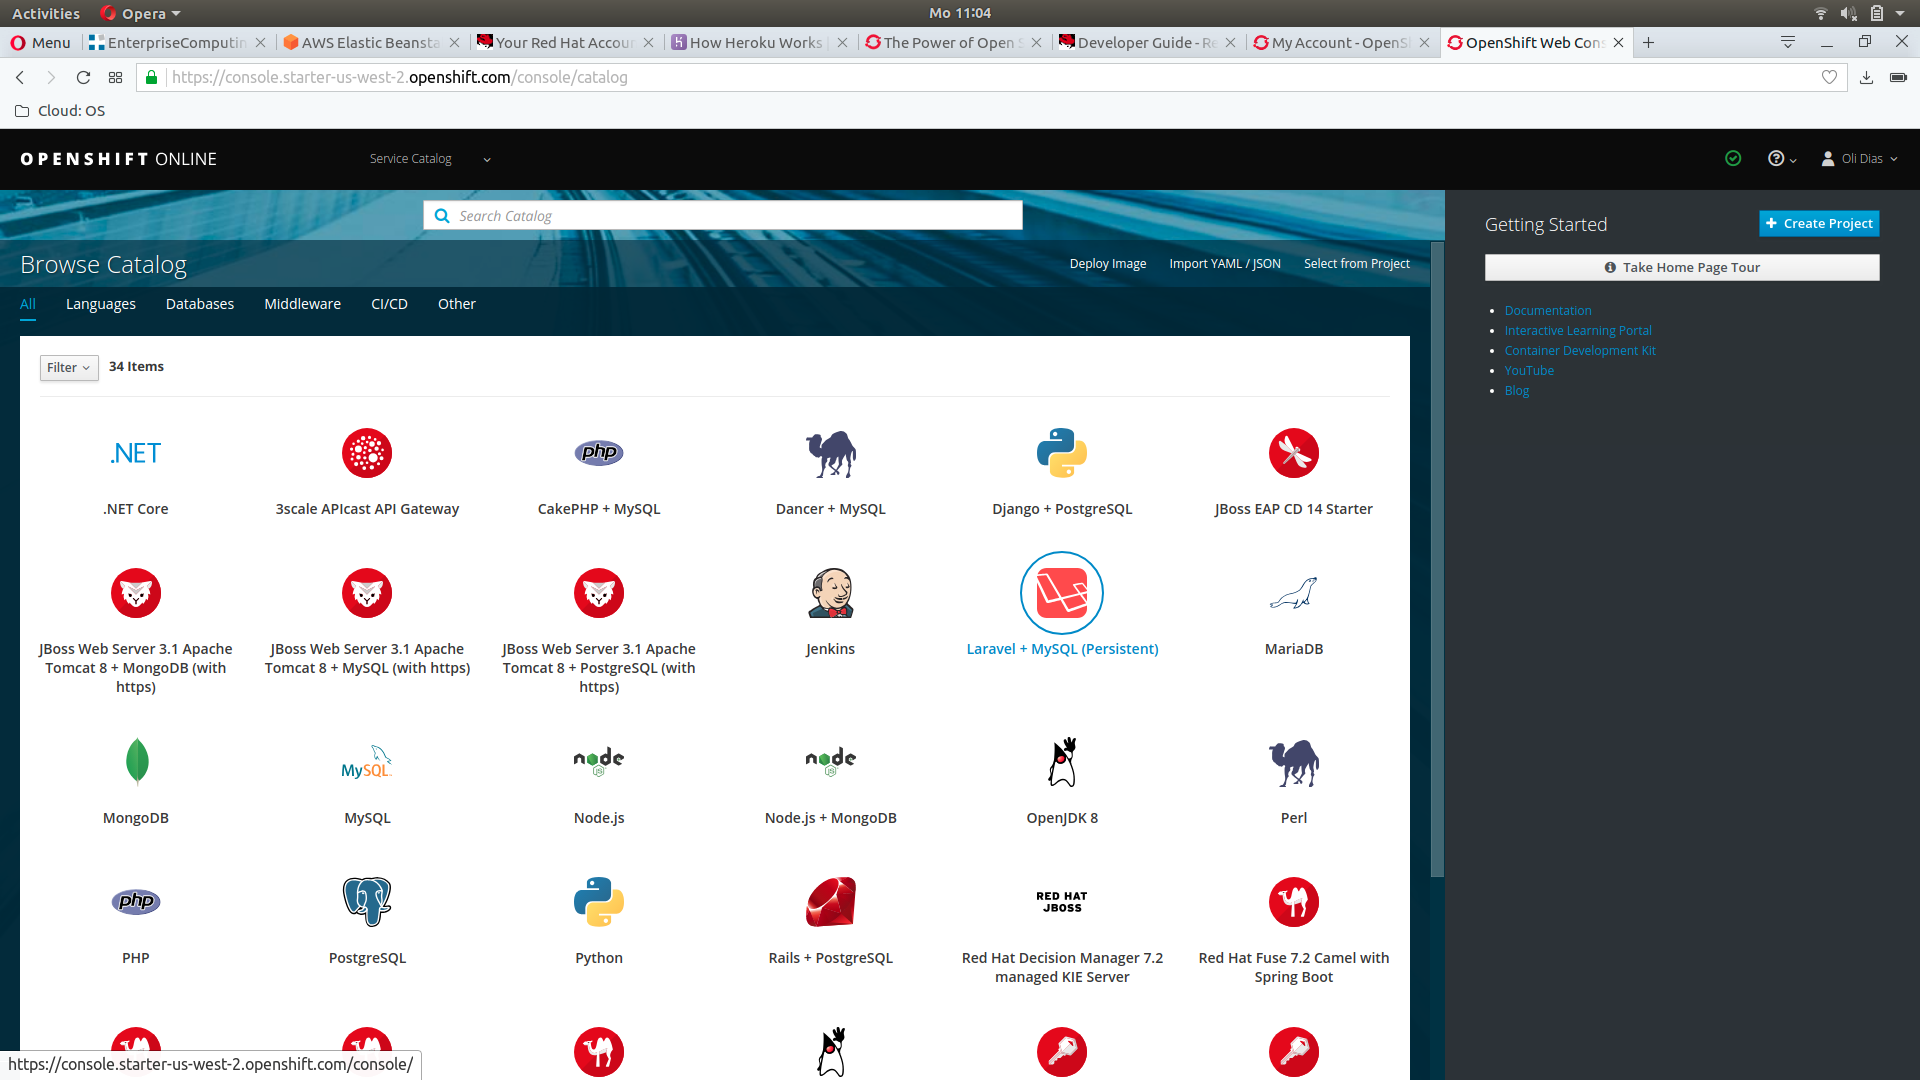
\includegraphics[width=0.7\linewidth]{img/os-overview-catalog}
	\caption{Auswahlkatalog aller möglichen Projekttypen}
	\label{fig:os-catalog}
\end{figure}

\begin{figure}%
    \centering
    \subfloat[Setup Dialog Schritt 1]{{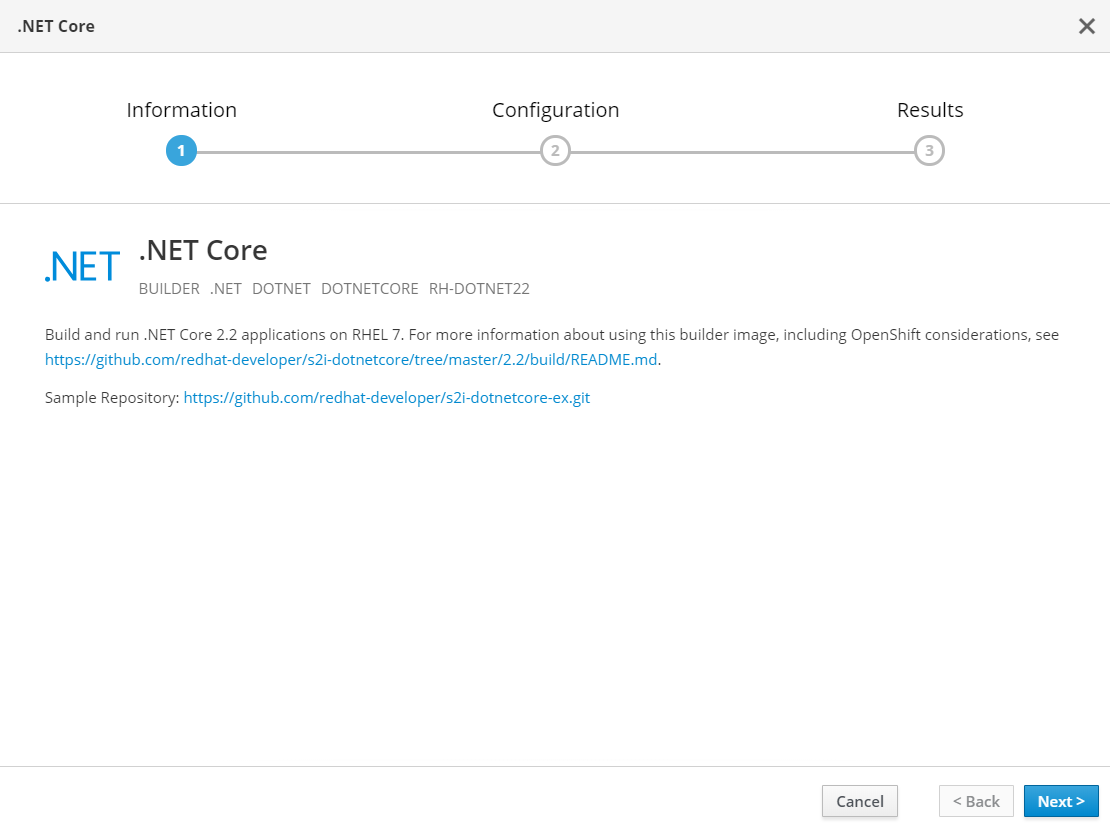
\includegraphics[width=5cm]{img/os-project-setup-1} }}%
    \qquad
    \subfloat[Setup Dialog Schritt 2]{{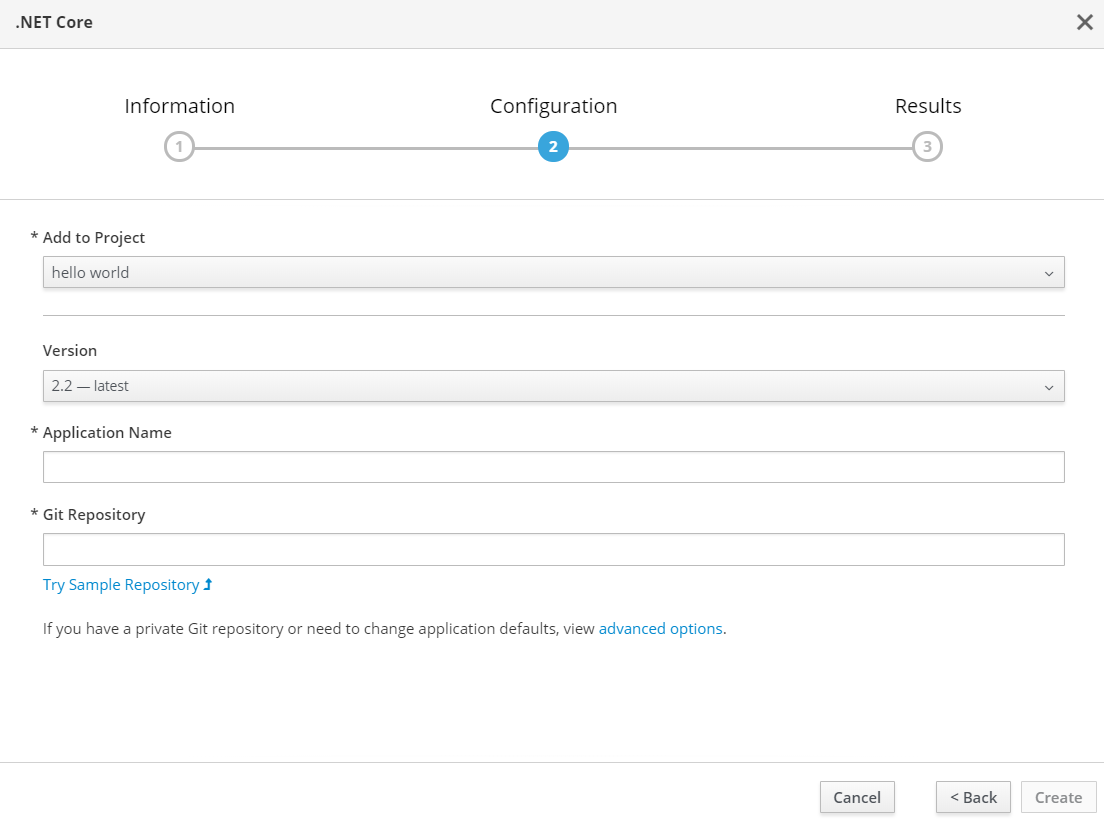
\includegraphics[width=5cm]{img/os-project-setup-2} }}
    \label{fig:os-setup}%
\end{figure}

Die Projektübersicht bietet nebst einigen generellen Informationen die Möglichkeit zum Build und Deployment.

\begin{figure}[h]
	\centering
	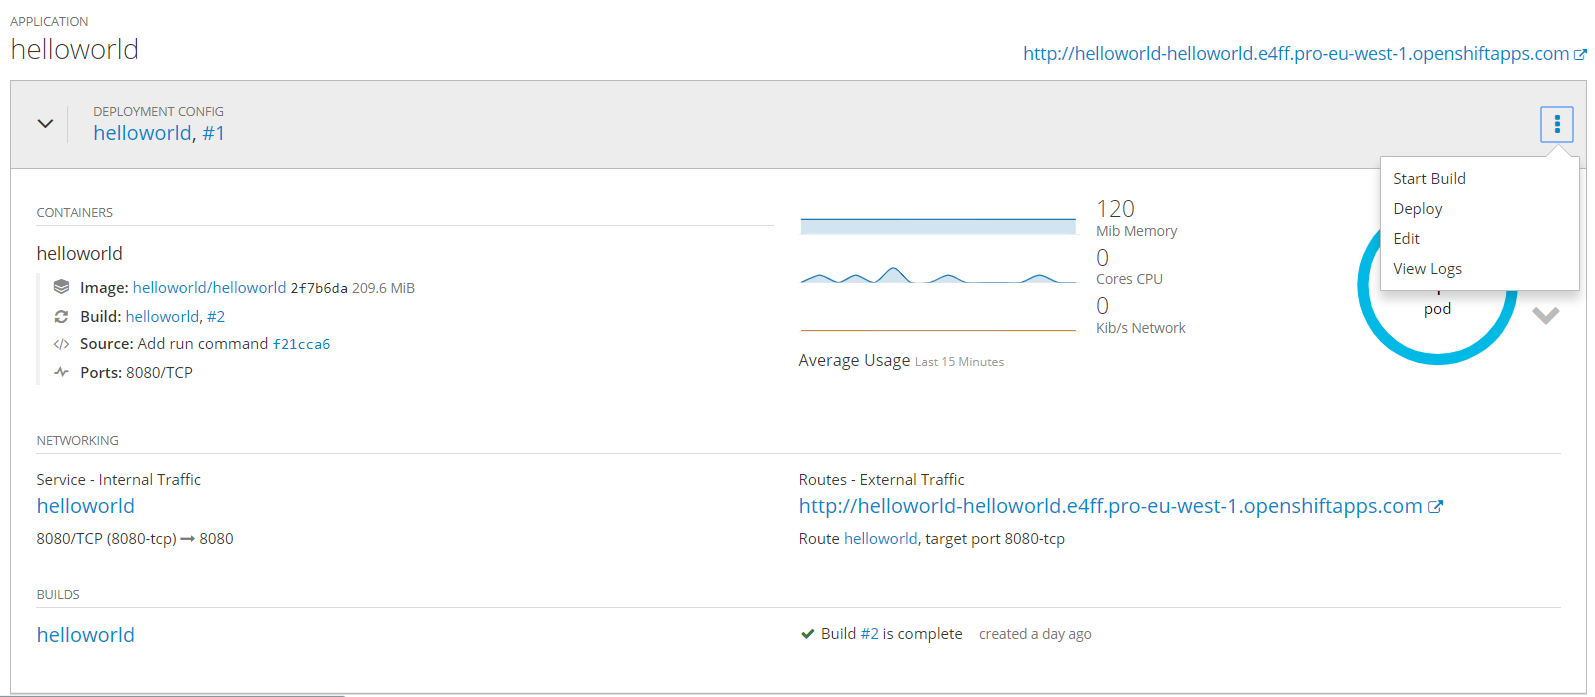
\includegraphics[width=0.7\linewidth]{img/os-project-overview}
	\caption{Ansicht der Projektübersicht}
	\label{fig:os-project-overview}
\end{figure}

\subsection{Scalable}

Die Nutzung von Openshift erfordert, dass man sich für ein Abonnement entscheidet. Nebst den kostenlosen Einführungsangeboten bedarf die langfristige Nutzung das Abonnement "OpenShift Online Pro". Im Standard bekommt man hierfür folgende Ressourcen:

\begin{itemize}
	\item 10 Projects
	\item 2 GB Memory
	\item 2 GB Terminating Memory
	\item 2 GB Storage
\end{itemize}

Um mehr als 10 Projekte zu verwalten bedarf es einem neuen Abonnement. Falls mehr Arbeitsspeicher oder Speicher nötig ist, kann das aktuelle Abonnement angepasst werden, was natürlich einen Einfluss auf den Preis hat. Trotzdem gibt es folgende Begrenzungen:

\begin{itemize}
	\item Arbeitsspeicher: maximal 48 GB
	\item Speicher: maximal 150 GB
\end{itemize}

\begin{figure}[h]
	\centering
	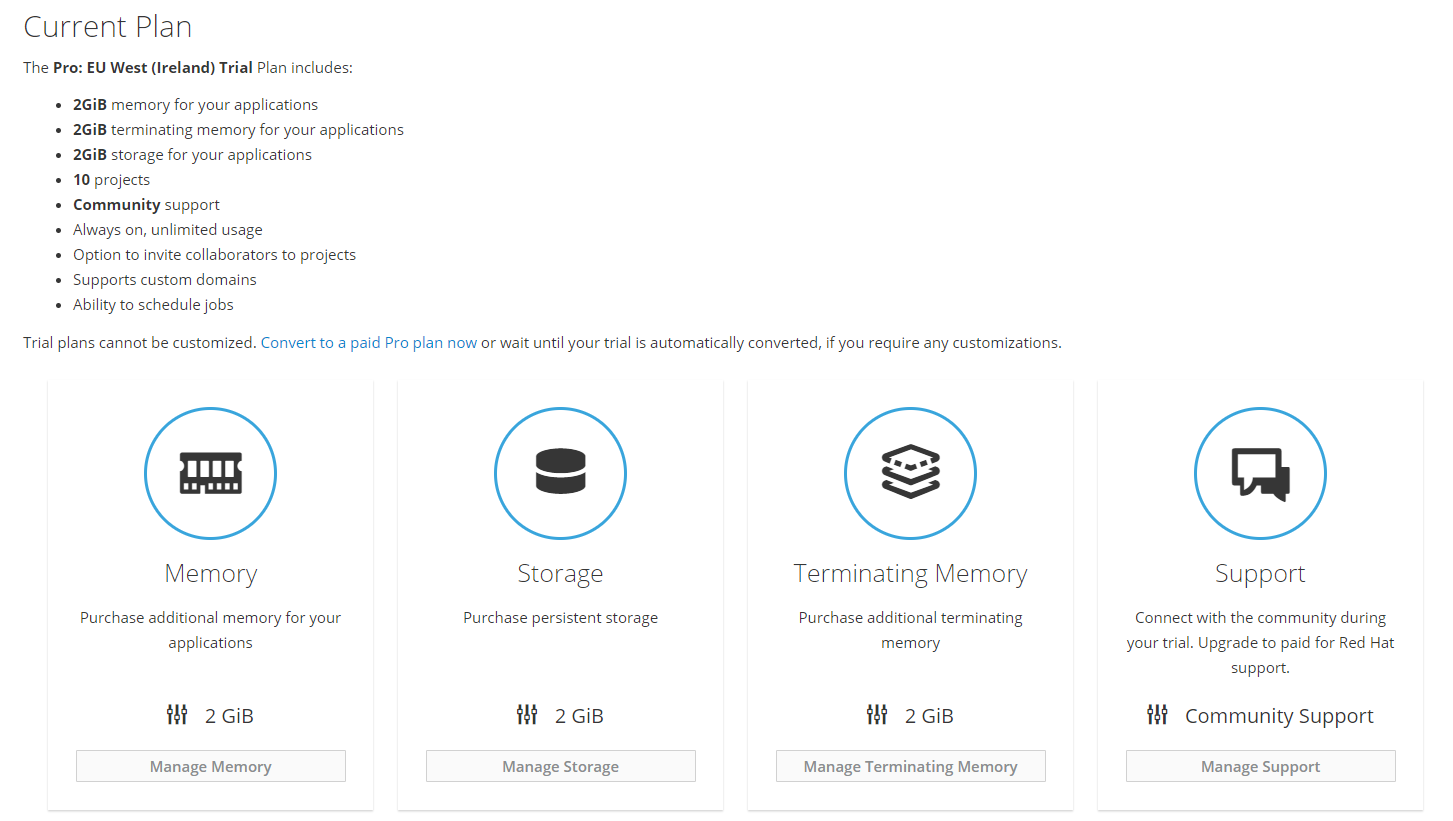
\includegraphics[width=0.7\linewidth]{img/os-scalability}
	\caption{Verwaltung der Ressourcen eines Abonnements}
	\label{fig:os-scalability}
\end{figure}

\subsection{Measurable}

Die aktuelle Nutzung der Ressourcen kann lediglich auf Projektstufe eingesehen werden. Diese Übersicht ist ziemlich einfach gehalten, ledicglich genutzer Arbeitsspeicher und Speicher werden im Verhältnis zum Maximum angezeigt.

\begin{figure}[h]
	\centering
	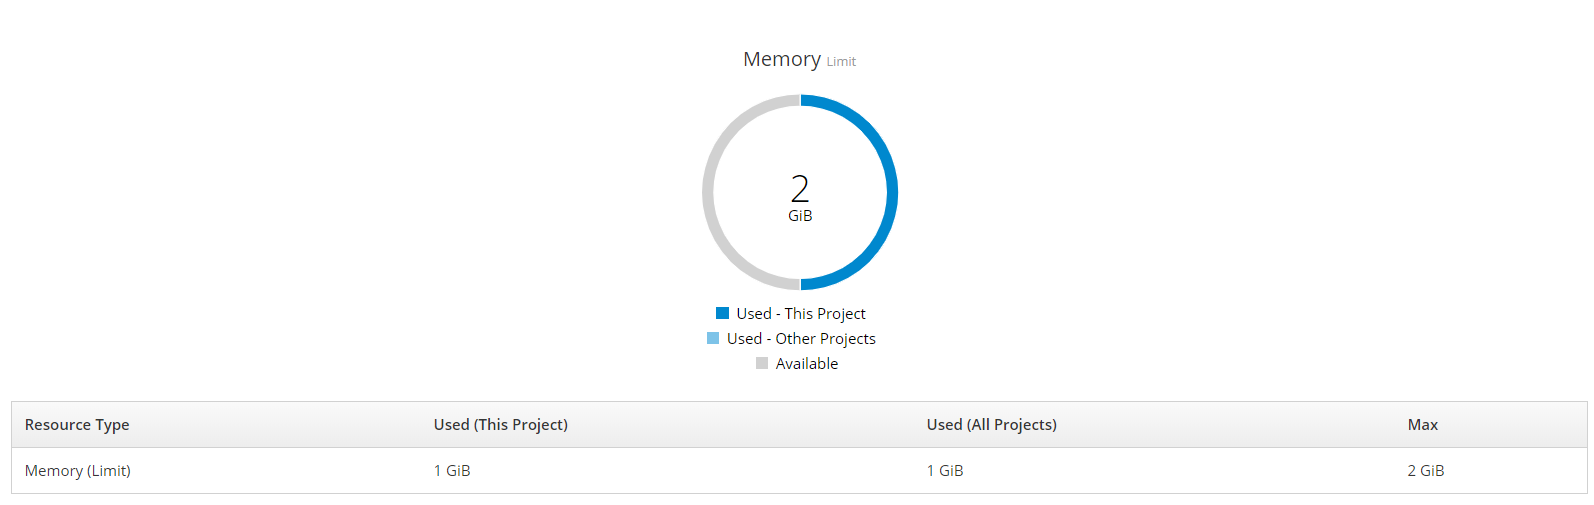
\includegraphics[width=0.7\linewidth]{img/os-quota}
	\caption{Übersicht der genutzten Ressourcen}
	\label{fig:os-quota}
\end{figure}

\section{Konzept: Cloud Computing Patterns}

Openshift bietet Entwicklern mit dem Konzept PaaS eine Plattform an, auf welcher eine App relative einfach deployed werden kann. Dies bringt den Vorteil, dass der Entwickler sich nicht mit der Komplexität der Building-/Deploying Infrastruktur auseinandersetzen muss.
Die Applikation läuft anschliessend auf sogenannten "Pods", welche vergleichbar mit Docker-Container sind. Einerseits kann die Anzahl Pod's pro Projekt manuell festeglegt und geändert werden. Zudem gibt es die Mgölichkeit für Pod Autoscaling. Sobald ein Pod bis zu
einem gewissen Grad ausgelastet wird, kommt ein zusätzlicher Pod in Aktion, sofern die maximale Anzahl definierter Pod's nicht erreicht wurde.

\begin{figure}[h]
	\centering
	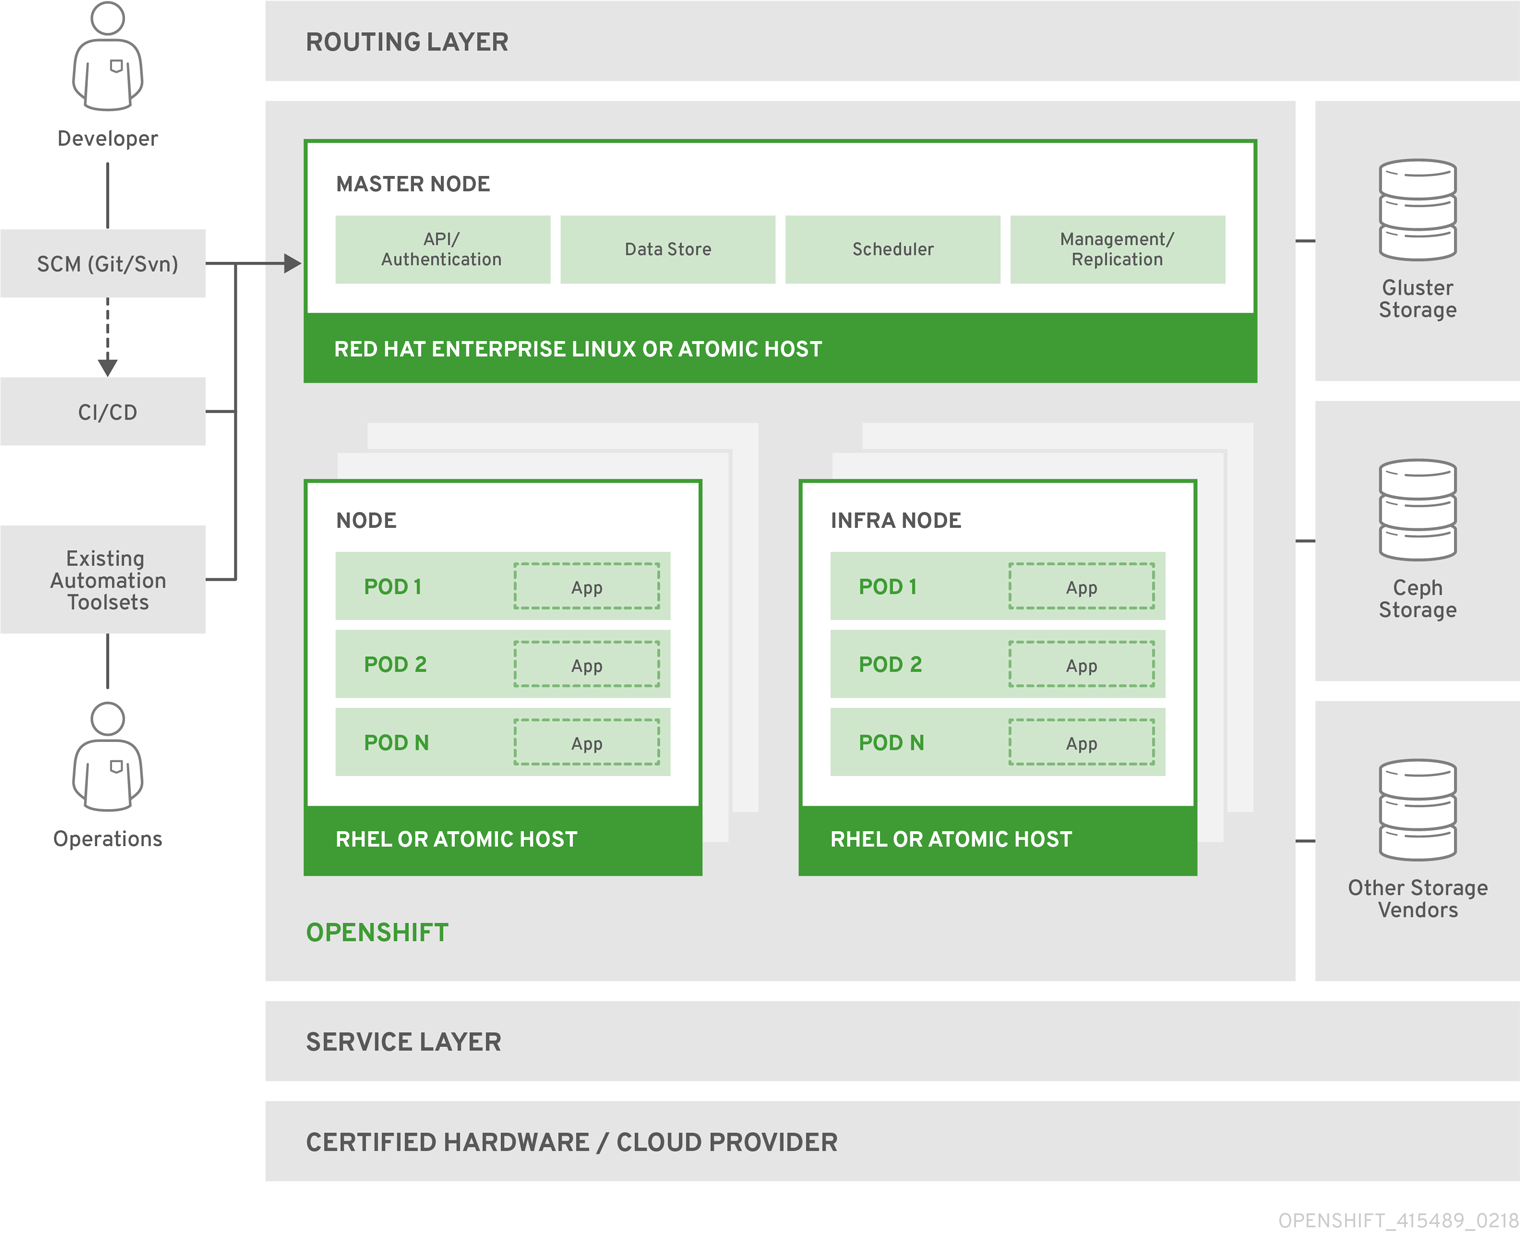
\includegraphics[width=0.7\linewidth]{img/os-architecture}
	\caption{Architekturübersicht der Openshift-Plattform}
	\label{fig:os-architecture}
\end{figure}

\section{Hands-On: Self Information}
Für das Deployment der gegebenen Self-Information Spring Applikation sind ähnliche Schritte wie schon bei der ASP.NET Core Applikation notwendig. Da es sich um eine Java Applikation handelt, muss auf jedenfall eine JVM auf dem Zielrechner existieren. Der Applikationserver Wildfly bietet eine gute Umgebung inklusive JVM (Oracle), auf welcher unsere Applikation ausgeführt wird. 

\subsection{Vorgehen}
Analog zu Kapitel \ref{sec:net-webui} muss zuerst ein Projekt erstellt werden. Wie erwähnt wählen wir hier aber ein Wildfly-Projekt. Nachdem die nötigen Informationen ausgefüllt wurden, muss das Projekt mit dem GitHub Repository verknüpft werden. Optional kann ein Webhook konfiguriert werden, mit welchem der CI/CD-Prozess nach einem Push auf das Repository automatisch angestossen wird. 

Nach dem Erstellen und Verknüpfen des Projektes wird der initale Build und das Deployment automatisch getriggered. Ohne weitere Konfiguration für Openshift wird nun ein Wildfly Applikationsserver aufgezogen und gestartet. Wir müssen jetzt Openshift so konfigurieren, dass das Jar-File vom Build der Spring Applikation ausgeführt und geroutet wird. Dazu reicht ein \texttt{run} File im Ordner \texttt{.s2i/bin} mit folgendem Inhalt:
\begin{lstlisting}[breaklines=true]
exec java -jar /wildfly/standalone/deployments/self-information-0.0.1-SNAPSHOT.jar
\end{lstlisting}
Mit diesem Befehl wird nach dem Aufziehen des Applikationsserver die Spring Applikation gestartet. Anstelle des absoluten Pfades wäre es denkbar, den Pfad des Jar-Files in eine Openshift-Umgebungsvariable zu speichern. 

Nach diesen Schritten sollte die Spring Applikation erfolgreich deployt sein. Im Web-UI kann die URL unter 'Application Console' $\rightarrow$ 'Applications' $\rightarrow$ 'Routes' $\rightarrow$ 'Hostname' gefunden werden. 

\subsection{Zusatzinformationen}
In der Standardkonfiguration des Pro-Abonnements von Openshift Cloud sind bis zu 2 GiB RAM sowie 10 GiB Storage enthalten. Die Self-Information Applikation verbraucht davon ca. 260MiB RAM verteilt auf 2 Pods. Gemäss der laufenden Applikation ist die IP 10.129.29.151.

\begin{figure}[h]
	\centering
	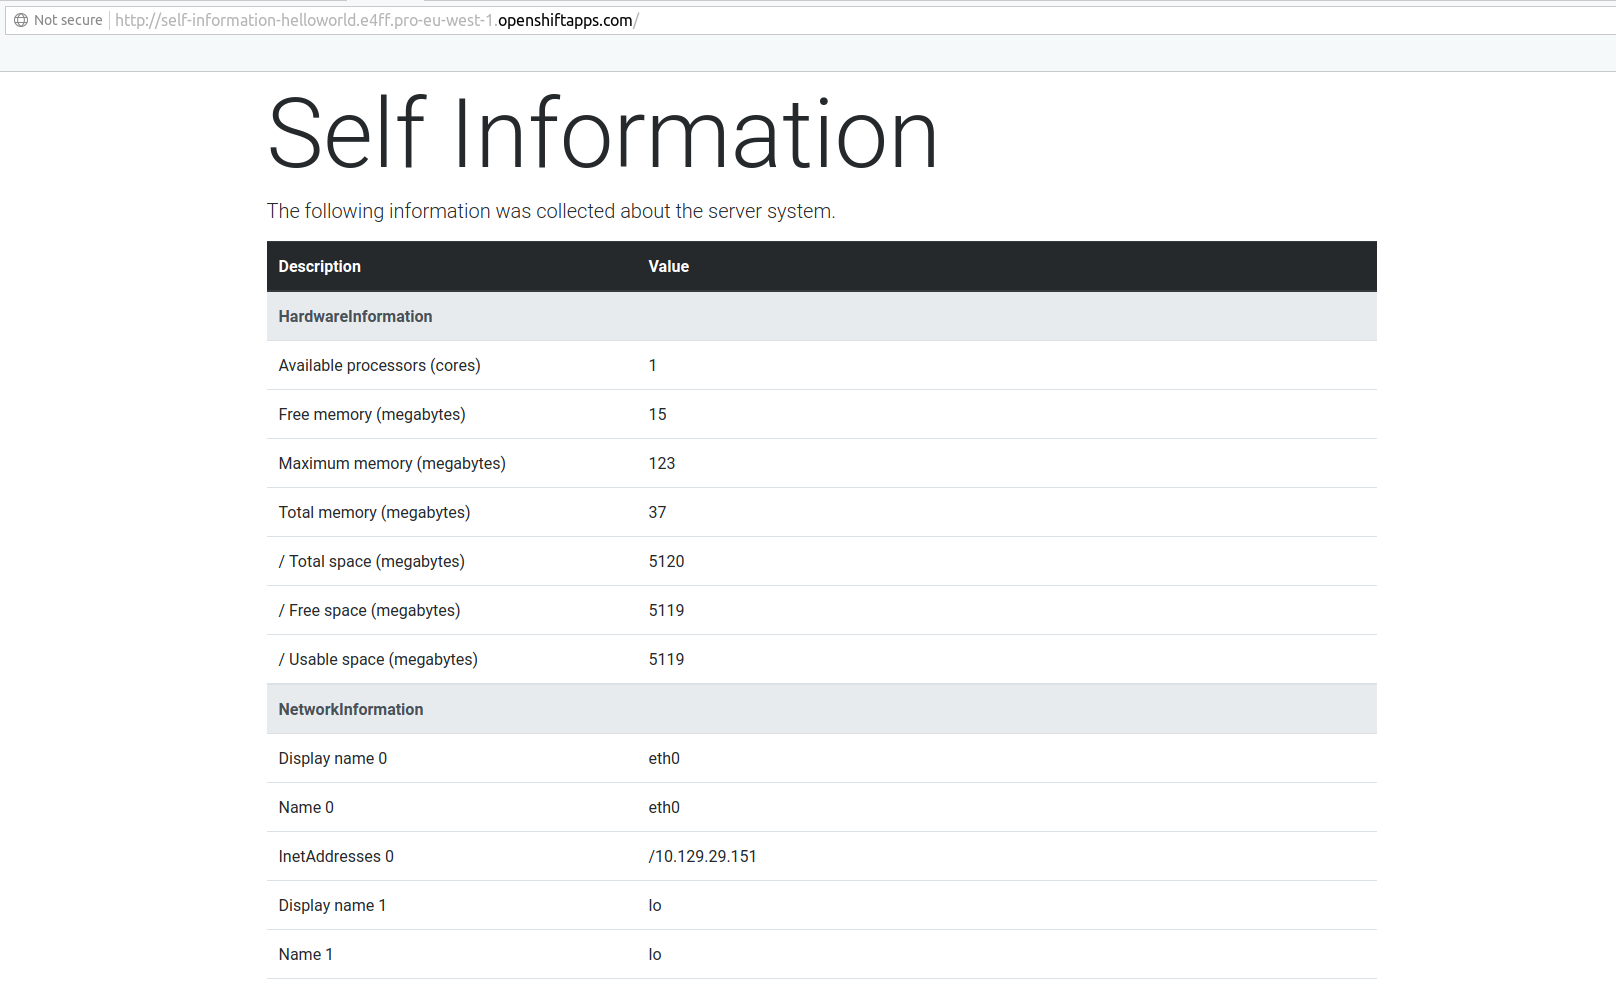
\includegraphics[width=1\linewidth]{img/self-information}
	\caption{Self-Information Screenshot}
	\label{fig:self-information}
\end{figure}


\section{Analyse: Preisrecherche}
%TODO Welche Preismodelle stehen zur Verfügung (Bsp. Subscription, Flat Rate, Pay-per-Use)?
%Wie kann bezahlt werden (Kreditkarte, Rechnung, ...)?
%Gibt es ein Gratis-Angebot für Einsteiger (falls ja: was sind %die Einschränkungen)?
%Welche Ressourcen werden abgerechnet?
%Was kostet Sie das Hosting der Anwendung aus der Ausgangslage?
%Vergleichen Sie das im vorherigen Schritt gefundene Angebot mit Amazon Web Services
%(AWS) Elastic Compute Cloud (EC2) anhand des AWS-Preiskalkulators. 3
%Welche Schwierigkeiten treten bei den Vergleich auf (z.B. unterschiedliche Servicemodelle
%oder Qualitätseigenschaften, versteckte Kosten, widersprüchliche Angaben)?

\subsection{Preismodelle}
Openshift bietet dem Endnutzer nur einige wenige Möglichkeiten am, um ihre Dienste nutzen zu können. Für die geschilderte Ausgangslage bedarf es einer Subskription für den Plan Openshift Online Pro mit zusätzlichen Ressourcen. Openshift bietet in ihrem Standard des
Pro Plans lediglich 2 GB RAM und 2 GB Speicher zur Verfügung. Der Erwerb der zusätzlichen Ressourcen führt zu einem monatlichen Kostenpunkt von 118 Dollar. Nebst RAM und Speicher werden terminierter Speicher (welcher nur temporär z.B. für das Builden gebraucht wird)
und Support als Ressourcen erworben werden.

\subsection{Zahlungsmöglichkeiten}
Der Rechnungsbetrag kann lediglich mit Kreditkarte beglichen werden, welche beim Kauf hinterlegt werden muss. Um sich lediglich ein Bild der Plattform machen zu können bietet Openshift kostenlos einen 30-tägigen Testzugang an.

\subsection{Vergleich Amazon EC2}
Vergleichsweise lässt sich bei Amazon ein Rechner mit ähnlichen Konfigurationen für jährlich 990 Dollar mieten, was ziemlich nahe dem monatlichen Preis von Openshift kommt. Die Schwierigkeit des Vergleichs besteht darin, dass sich die Angebot vieler Provider unterscheiden.
Bei Openshift hat man die Freiheit, die Ressourcen sehr genau selbst definieren zu können, wogleich bei Amazon vordefinierte Pakete von Rechner geschnürt wurden.

\section{Analyse: Preisvergleich eigenes Hosting, IaaS und PaaS}

\subsection{Kostenaufstellung}
Mit der geschilderten Ausgangslage wurden folgende Annahmen getroffen:

\begin{itemize}
	\item Beschaffungskosten eigener Server: 1'000
	\item Server Administrationskosten pro Jahr: 8'000 (10\% Stelle mit Ansatz 80'000 Jahresgehalt)
\end{itemize}

Daraus ergibt sich folgende Kostenaufstellung:

\begin{table}[H]
    \begin{tabular}{| l | l | l | l | l |}
		\hline
        Kostenart & Eigener Server & Google & Amazon E2C & Openshift \\ \hline
        Beschaffung & 1'000 & 3'800 & 3'600 & 13'200\\
        Betrieb & 16'000 & 4'000 & 4'000 & 4'000\\
        Total & 17'000 & 7'800 & 7'600 & 17'200 \\ \hline
    \end{tabular}
    \caption{Vergleich zwischen lokalen Servern und Cloud Servern}
\end{table}

\subsection{Fazit}
Im Vergleich schneiden die beiden grossen Cloud Provider Amazon und Google am besten ab. Mit etwas Interpretation lässt sich jedoch erkennen, dass die totalen Kosten stark abhängig von der Anzahl Servern ist.
Das heisst, je mehr Server für eine Applikation gebraucht werden, umso mehr lohnt sich die Investition in eine eigene Infrastruktur.

Ein weiterer Aspekt stellt die Vertraulichkeit der Applikationsdaten dar. So erwartet der normale Kunde einer Bank, dass seine Kreditkarteninformationen nicht bei einem Server eines externen Anbieters taummeln.

Generell macht es Sinn, Cloud Provider nach den benötigten Funktionalitäten einzuschränken und erst in einem zweiten Schritt preistechnisch zu optimieren. Eine Herausforderung stellt hierbei der Vergleich der einzelnen Provider dar.
Oftmals haben unterschiedliche Provider verschieden Angebote mit unterschiedlichen Konfigurationen, was einen direkten Vergleich erschwert.

\end{document}
